% phpcpd-next — academic paper
% Build: bash bin/build-paper.sh   (or: pdflatex paper.tex ; pdflatex paper.tex)
%
% STYLE CONVENTIONS (keep consistent when editing):
%   Prose  — Strunk & White: omit needless words, active voice, parallel lists,
%            precise diction (no slang).
%   Numbers — Chicago Manual of Style 16.10 alternative (technical) rule:
%            * spell out single-digit counts in running prose (two methods, six corpora);
%            * use numerals for 10 and above, and within a category keep them
%              consistent (e.g. "17 ... to 0");
%            * always numerals for percentages, measurements, math-mode quantities,
%              edit-distance costs/budgets, CLI literal values, versions, table data,
%              and designators (Type-3, level 10, R1, v6.0.3);
%            * never begin a sentence with a numeral.
\documentclass[10pt,a4paper]{article}

\usepackage[utf8]{inputenc}
\usepackage[T1]{fontenc}
\usepackage{lmodern}
\usepackage[margin=1in]{geometry}
\usepackage{amsmath,amssymb}
\usepackage{booktabs}
\usepackage{multirow}
\usepackage{makecell}
\usepackage{array}
\usepackage{xcolor}
\usepackage{caption}
\usepackage{subcaption}
\usepackage{listings}
\usepackage{enumitem}
\usepackage{titlesec}
\usepackage{microtype}
\usepackage{pgfplots}
\usepackage{pgfplotstable}

% The measured tables are read, not retyped. bench/results/compare.tsv is
% derived from bench/results/compare/*.tsv by bench/build-tables.php, and
% bench/results/walltime.tsv is written by bench/check-walltime.php itself.
% Both the plot and the tabular below read those files, so a re-measurement
% updates the artefact rather than leaving it to be transcribed a third time.
\pgfplotstableread[col sep=tab]{../../bench/results/compare.tsv}\comparedata
\pgfplotstableread[col sep=tab]{../../bench/results/e2/summary.tsv}\etwodata
\pgfplotstableread[col sep=tab]{../../bench/results/out-of-the-box.tsv}\oobdata

% Measured values, generated by bench/collect-facts.php. Numbers this paper
% would otherwise type out are read from here, for the same reason its plots
% read compare.tsv: a number that is fetched cannot be out of date, and an
% undefined macro stops the build where a stale figure would not.
% Generated by bench/collect-facts.php. Do not edit.
%
% Measured values, for a document that would otherwise type them out.
% An undefined macro is a build error; a stale number is not, which is why
% the paper reads these rather than keeping copies of them.

\newcommand{\factScanCorpusFilesTotal}{6714}
\newcommand{\factScanFireflyIiiFiles}{1445}
\newcommand{\factScanFireflyIiiSkipped}{0}
\newcommand{\factScanPhpParserFiles}{340}
\newcommand{\factScanPhpParserSkipped}{2}
\newcommand{\factScanPhpunitFiles}{2689}
\newcommand{\factScanPhpunitSkipped}{1}
\newcommand{\factScanSymfonyConsoleFiles}{359}
\newcommand{\factScanSymfonyConsoleSkipped}{0}
\newcommand{\factScanSymfonyStringFiles}{33}
\newcommand{\factScanSymfonyStringSkipped}{0}
\newcommand{\factScanWordpressFiles}{1848}
\newcommand{\factScanWordpressSkipped}{3}
\newcommand{\factCodeDisplacedMassFloor}{16}
\newcommand{\factCodeMinimumMinTokens}{38}
\newcommand{\factCodeNormalizedDiversityFloor}{3}
\newcommand{\factCodePerFileCap}{32}
\newcommand{\factCodePostingsCap}{1000}
\newcommand{\factCodePostingsPairs}{499500}
\newcommand{\factCodeRatio}{0.15}
\newcommand{\factCodeRelease}{2.0.0}
\newcommand{\factCodeSeedLength}{16}
\newcommand{\factCodeSeedPairCap}{16000}
\newcommand{\factCodeShingleLength}{3}
\newcommand{\factCodeSimilarityFloor}{0.85}
\newcommand{\factCodeTheta}{0.7}
\newcommand{\factCodeVersion}{2.0.0}
\newcommand{\factWalltimeFireflyIiiClones}{961}
\newcommand{\factWalltimeFireflyIiiDefault}{4.606}
\newcommand{\factWalltimeFireflyIiiDefaultspread}{0.152}
\newcommand{\factWalltimeFireflyIiiFiles}{1291}
\newcommand{\factWalltimeFireflyIiiFingerprint}{091a4704edf2-d8cf9b6c6256-1291}
\newcommand{\factWalltimeFireflyIiiRabinkarp}{1.884}
\newcommand{\factWalltimeFireflyIiiRatio}{11.58}
\newcommand{\factWalltimeFireflyIiiTokenbag}{2.779}
\newcommand{\factWalltimeFireflyIiiTriage}{2.164}
\newcommand{\factWalltimeFireflyIiiUnified}{53.319}
\newcommand{\factWalltimeFireflyIiiUnifiedspread}{3.311}
\newcommand{\factWalltimePhpParserClones}{78}
\newcommand{\factWalltimePhpParserDefault}{0.390}
\newcommand{\factWalltimePhpParserDefaultspread}{0.006}
\newcommand{\factWalltimePhpParserFiles}{340}
\newcommand{\factWalltimePhpParserFingerprint}{091a4704edf2-75cc5ec6b471-340}
\newcommand{\factWalltimePhpParserRabinkarp}{0.311}
\newcommand{\factWalltimePhpParserRatio}{8.08}
\newcommand{\factWalltimePhpParserTokenbag}{0.078}
\newcommand{\factWalltimePhpParserTriage}{0.362}
\newcommand{\factWalltimePhpParserUnified}{3.149}
\newcommand{\factWalltimePhpParserUnifiedspread}{0.019}
\newcommand{\factWalltimePhpunitClones}{923}
\newcommand{\factWalltimePhpunitDefault}{3.719}
\newcommand{\factWalltimePhpunitDefaultspread}{0.095}
\newcommand{\factWalltimePhpunitFiles}{2689}
\newcommand{\factWalltimePhpunitFingerprint}{091a4704edf2-8c702a30d091-2689}
\newcommand{\factWalltimePhpunitRabinkarp}{2.302}
\newcommand{\factWalltimePhpunitRatio}{31.90}
\newcommand{\factWalltimePhpunitTokenbag}{1.604}
\newcommand{\factWalltimePhpunitTriage}{2.389}
\newcommand{\factWalltimePhpunitUnified}{118.650}
\newcommand{\factWalltimePhpunitUnifiedspread}{5.121}
\newcommand{\factWalltimeSymfonyConsoleClones}{234}
\newcommand{\factWalltimeSymfonyConsoleDefault}{0.951}
\newcommand{\factWalltimeSymfonyConsoleDefaultspread}{0.049}
\newcommand{\factWalltimeSymfonyConsoleFiles}{359}
\newcommand{\factWalltimeSymfonyConsoleFingerprint}{091a4704edf2-e85d64fa990e-359}
\newcommand{\factWalltimeSymfonyConsoleRabinkarp}{0.717}
\newcommand{\factWalltimeSymfonyConsoleRatio}{9.32}
\newcommand{\factWalltimeSymfonyConsoleTokenbag}{0.240}
\newcommand{\factWalltimeSymfonyConsoleTriage}{0.845}
\newcommand{\factWalltimeSymfonyConsoleUnified}{8.858}
\newcommand{\factWalltimeSymfonyConsoleUnifiedspread}{1.294}
\newcommand{\factWalltimeSymfonyStringClones}{50}
\newcommand{\factWalltimeSymfonyStringDefault}{0.212}
\newcommand{\factWalltimeSymfonyStringDefaultspread}{0.040}
\newcommand{\factWalltimeSymfonyStringFiles}{33}
\newcommand{\factWalltimeSymfonyStringFingerprint}{091a4704edf2-9d02089f5087-33}
\newcommand{\factWalltimeSymfonyStringRabinkarp}{0.154}
\newcommand{\factWalltimeSymfonyStringRatio}{10.46}
\newcommand{\factWalltimeSymfonyStringTokenbag}{0.029}
\newcommand{\factWalltimeSymfonyStringTriage}{0.156}
\newcommand{\factWalltimeSymfonyStringUnified}{2.221}
\newcommand{\factWalltimeSymfonyStringUnifiedspread}{0.339}
\newcommand{\factWalltimeWordpressClones}{1389}
\newcommand{\factWalltimeWordpressDefault}{29.041}
\newcommand{\factWalltimeWordpressDefaultspread}{1.162}
\newcommand{\factWalltimeWordpressFiles}{1848}
\newcommand{\factWalltimeWordpressFingerprint}{091a4704edf2-4fcf7813b552-1848}
\newcommand{\factWalltimeWordpressRabinkarp}{8.085}
\newcommand{\factWalltimeWordpressRatio}{3.44}
\newcommand{\factWalltimeWordpressTokenbag}{21.488}
\newcommand{\factWalltimeWordpressTriage}{9.991}
\newcommand{\factWalltimeWordpressUnified}{99.889}
\newcommand{\factWalltimeWordpressUnifiedspread}{3.894}
\newcommand{\factPathsLogicShareTable}{bench/results/logic-share-table.txt}
\newcommand{\factPathsWalltimeTable}{bench/results/walltime-table.txt}
\newcommand{\factAliasPerFileCap}{fingerprint file cap seed}
\newcommand{\factAliasPostingsCap}{corpus fingerprint posting}
\newcommand{\factAliasPostingsPairs}{pairs seed corpus}
\newcommand{\factAliasSeedLength}{winnowing window token K}
\newcommand{\factAliasSeedPairCap}{pairs seed enumerated}
\newcommand{\factAliasSimilarityFloor}{similarity emission invariant}
\newcommand{\factAliasTheta}{similarity sim}
\newcommand{\factProvenanceScanMachine}{cpu=Intel(R) Core(TM) i7-8650U CPU @ 1.90GHz governor=powersave epp=power power=battery clock=800/4200MHz load=1.37/8 cpus}
\newcommand{\factProvenanceScanMeasuredAt}{2026-09-13}
\newcommand{\factProvenanceWalltimeMachine}{cpu=Intel(R) Core(TM) i7-8650U CPU @ 1.90GHz governor=powersave epp=performance power=AC clock=3300/4200MHz load=2.21/8 cpus}
\newcommand{\factProvenanceWalltimeMeasuredAt}{2026-09-10}

\pgfplotsset{compat=1.16}
\usepgfplotslibrary{statistics}
\usetikzlibrary{patterns}

% ---- monochrome palette: grayscale shades for figures, one tone for links ----
\definecolor{g1}{gray}{0.00}
\definecolor{g2}{gray}{0.35}
\definecolor{g3}{gray}{0.60}
\definecolor{g4}{gray}{0.82}
\definecolor{linkmono}{gray}{0.30}

\usepackage[colorlinks=true,allcolors=linkmono]{hyperref}

% ---- listings: uniform monospace, no syntax colouring (mono pattern throughout) ----
\lstset{
  basicstyle=\ttfamily,
  columns=fullflexible,
  keepspaces=true,
  breaklines=true,
  breakatwhitespace=true,
  showstringspaces=false,
  frame=single,
  framesep=4pt,
  rulecolor=\color{black!35},
}

% lightweight theorem-like environments without amsthm dependency
\newcounter{defn}[section]
\newcommand{\defn}[1]{\par\medskip\refstepcounter{defn}%
  \noindent\textbf{Definition~\thedefn} (#1)\textbf{.}\ }
\newcounter{prop}[section]
\newcommand{\prop}[1]{\par\medskip\refstepcounter{prop}%
  \noindent\textbf{Proposition~\theprop} (#1)\textbf{.}\ \itshape}
\newcounter{lem}[section]
\newcommand{\lem}[1]{\par\medskip\refstepcounter{lem}%
  \noindent\textbf{Lemma~\thelem} (#1)\textbf{.}\ \itshape}

\titleformat{\section}{\large\bfseries}{\thesection}{0.6em}{}
\titleformat{\subsection}{\normalsize\bfseries}{\thesubsection}{0.6em}{}

\setlength{\parskip}{2pt}
\setlength{\parindent}{1.2em}
% absorb minor overfulls from long unbreakable code identifiers
\setlength{\emergencystretch}{3em}

\title{\textbf{Token-Based Clone Detection for PHP:\\
An Empirical Evaluation of Methods and a Labelled Benchmark}}

\author{Luciano Federico Pereira\\[2pt]
\small ORCID: \href{https://orcid.org/0009-0002-4591-6568}{0009-0002-4591-6568}}

\date{June 2026}

\begin{document}
\maketitle

\begin{abstract}
\noindent
\texttt{phpcpd} is a widely used PHP copy/paste detector whose last released version (6.0.3, 2020)
performs Rabin--Karp exact matching of Type-1 and Type-2 clones. A subsequent, unreleased 7.0.0
development line added a ConQAT-style approximate suffix-tree algorithm for Type-3 (near-miss)
detection (contributed upstream as pull request~\#199); however, 7.0.0 was never released and the
project was archived in 2023, so this capability did not reach users. The clone-detection literature
offers further methods --- order-invariant token-bag matching and type-aware normalization --- that
had not been applied to PHP, and, unlike Java (BigCloneBench) or C (POJ-104), no labelled PHP clone
benchmark existed on which to evaluate any of them. This paper reports an empirical study based on the
archived \texttt{phpcpd} codebase. We (i)~modernize it reproducibly to PHP~8.5, PHPStan level~10, and a
159-test suite, and complete and evaluate its previously unreleased suffix-tree engine; (ii)~implement
additional literature-grounded methods as selectable engines --- a SourcererCC token-bag matcher,
type-aware edit weights, a token-type abstraction with a \texttt{-{}-type-anchored} variant, an IDF
stopword filter, and an incremental index that provably reproduces a full pass; and (iii)~construct
\textbf{BCB-PHP}, a labelled PHP clone benchmark (to our knowledge the first), comprising a
mutation-injection harness over a pinned, six-corpus type-density gradient. Evaluating each method on
BCB-PHP yields a type-density$\times$clone-density map, a specificity increase of $+1.9$ to $+18.9$
points from type-anchored normalization at no recall cost, and confirmed inconsistent clones in an
application corpus. The results motivate a combined exact-and-reorder-tolerant default configuration
(\texttt{rk+tb}); identifier fuzzing is shown to reduce precision substantially, and approximate
suffix-tree matching to be better suited to targeted analysis than to default use. BCB-PHP is released
for reuse; its type-density gradient supports further study of clone detection on modern typed versus
traditional untyped PHP and of differences between methods.
\end{abstract}

\section*{Note on revision (2026-09-15)}
\addcontentsline{toc}{section}{Note on revision}

Three of this paper's measurements described an engine that had since moved, and
are corrected in place rather than annotated: the comparison against the
original \texttt{phpcpd.phar} (\S\ref{sec:practical}), which a change to the
token model made incommensurable at a shared threshold; a boundary statistic
that turned out to measure its own instrument rather than the engine; and the
precision section (\S\ref{sec:precision-correction}), which gains a second
study on public corpora rather than losing the one it had. One configuration the paper recommended, \texttt{tb+fuzzy}, no longer
exists and the recommendation is withdrawn with its justification given below.
Every table in this paper is typeset from a committed result file rather than
transcribed, and each reproduces from the harness that wrote it. Nothing in the
conclusions changed direction.

\section{Introduction}

\texttt{phpcpd} is a carefully engineered PHP copy/paste detector developed by Sebastian Bergmann: a
Rabin--Karp rolling hash over a normalized token stream that hashes fixed windows, reports collisions,
and detects Type-1 and Type-2 clones. It is fast, dependency-light, and widely used. Its last released
version, 6.0.3 (2020), implements this single Rabin--Karp strategy and does not attempt Type-3
(near-miss/gapped) or reorder-tolerant detection --- an appropriate scope for an exact-match detector.

A subsequent development line did go further: an unreleased 7.0.0 added a ConQAT-style approximate
suffix-tree algorithm with a configurable edit budget for Type-3 detection~\cite{conqat}, contributed
upstream as pull request~\#199. That release, however, was never published --- its changelog entry
carries an unfilled date --- and the repository was archived in 2023, so the capability remained in the
codebase but absent from any release and unevaluated in practice. The clone-detection literature offers
further methods still: SourcererCC's order-invariant token-bag matching for reordered
code~\cite{sourcerercc} and Toma's token-type abstraction for stronger Type-2
normalization~\cite{toma}, neither of which had been applied to PHP. Evaluating any of these on PHP
faced a further obstacle: unlike Java (BigCloneBench~\cite{bigclonebench}) or C (POJ-104), no labelled
PHP clone benchmark existed.

\paragraph{Approach.} Building on the archived \texttt{phpcpd} codebase, we modernize it, complete and
evaluate its previously unreleased suffix-tree engine, implement additional literature-grounded
methods, and construct the benchmark required to evaluate them. We then determine empirically which
methods are appropriate for a default configuration in a fast command-line tool. The evaluation
indicates that a combined exact-and-reorder-tolerant configuration is the most suitable default, that
identifier fuzzing substantially reduces precision, and that approximate suffix-tree matching is better
reserved for targeted analysis.

\paragraph{Contributions.}
\begin{enumerate}[leftmargin=1.4em,itemsep=1pt,topsep=2pt]
  \item A \textbf{diff-level reproducible modernization} of an archived PHP tool to PHP~8.5, PHPStan
        level~10, PER-CS~2.0, and a 159-test suite, including the completion and first evaluation of
        \texttt{phpcpd}'s previously unreleased ConQAT suffix-tree engine (\S\ref{sec:method}).
  \item \textbf{Five detection methods implemented} as selectable engines on the inherited base: a
        SourcererCC token-bag matcher with IDF filtering, type-aware edit weights, an extended
        token-type abstraction with a type-anchored variant, inconsistent-clone reporting, and an
        incremental index --- each tied to a primary reference and an end-to-end test
        (\S\ref{sec:methods},~\S\ref{sec:engineering}).
  \item \textbf{BCB-PHP, a labelled PHP clone benchmark} (to our knowledge the first): a
        mutation-injection harness over a pinned, six-corpus type-density gradient (\S\ref{sec:eval}),
        released for reuse --- its gradient supports further study of modern typed vs.\ traditional
        untyped PHP and of method
        differences.
  \item An \textbf{empirical evaluation} on BCB-PHP yielding a type-density$\times$clone-density map, a
        $+1.9$ to $+18.9$ point specificity lift from type-anchored normalization at zero recall cost,
        a six-corpus method comparison, and real inconsistent clones in an application corpus
        (\S\ref{sec:eval}) --- from which we recommend the \texttt{rk+tb} default (\S\ref{sec:practical}).
\end{enumerate}

\section{Background: the phpcpd Codebase and Its Detection Methods}
\label{sec:methods}

\subsection{The released base engine (Rabin--Karp)}
phpcpd's last released version (6.0.3) provides a single strategy, \texttt{DefaultStrategy}, a
Rabin--Karp matcher. It normalizes tokens (whitespace and comments stripped; \texttt{-{}-fuzzy}
rewrites \lstinline!T_VARIABLE! to a placeholder), builds a per-token rolling signature, hashes fixed
windows of \texttt{-{}-min-tokens} tokens, and reports colliding windows filtered by
\texttt{-{}-min-lines}. It detects Type-1 and Type-2 exact-match clones and, by construction, tolerates
neither gaps nor reordering.

\subsection{The inherited suffix-tree engine (unreleased 7.0-dev)}
The repository's unreleased 7.0.0 line, which we fork, introduces a second strategy through a selector
in \texttt{Application.php} (upstream code; \texttt{tokenbag} is the only branch we add):

\begin{lstlisting}[basicstyle=\ttfamily\small]
return match ($algorithm) {                               // selector: upstream 7.0-dev
    null, 'rabin-karp' => new DefaultStrategy($config),    // phpcpd base engine
    'suffixtree'       => new SuffixTreeStrategy($config),  // upstream, PR #199
    'tokenbag'         => new TokenBagStrategy($config),    // added in phpcpd-next
};
\end{lstlisting}

The \texttt{SuffixTreeStrategy} $\rightarrow$ \texttt{ApproximateCloneDetectingSuffixTree} (an
implementation of the ConQAT algorithm~\cite{conqat}, contributed upstream as PR~\#199) tokenizes into
an \texttt{AbstractToken[]} word, appends a sentinel, builds a generalized suffix tree, and in
\lstinline!findClones($minLength, $maxErrors, $headEquality)! compares candidate token sequences by
\emph{approximate} match. A Levenshtein edit-distance matrix \lstinline!edBuffer! is maintained over
token sequences; a candidate extends only while the running edit distance stays $\le$ \texttt{maxErrors}
(the \texttt{-{}-edit-distance} flag, default~5), and \texttt{headEquality} enforces an exact-match
prefix before edits are allowed, as in ConQAT. Comparing by edit distance rather than hash equality,
this method detects Type-3 (near-miss/gapped) clones: inserted, deleted, or substituted statements
within the edit budget are tolerated. Because 7.0.0 was never released, this engine had not been
evaluated; we modernize it (\S\ref{sec:method}), repair two latent defects it exposed
(\S\ref{sec:engineering}), and evaluate it (\S\ref{sec:eval}).

\defn{token edit distance}
For token sequences $a_{1..m}$, $b_{1..n}$, the matcher fills $D$ with
\[
D[i,j]=\min\!\begin{cases}
D[i\!-\!1,j]+1 & \text{(deletion)}\\
D[i,j\!-\!1]+1 & \text{(insertion)}\\
D[i\!-\!1,j\!-\!1]+c(a_i,b_j) & \text{(match/substitution)}
\end{cases}
\]
and reports a clone while $\min_k D[\cdot,k]\le \texttt{maxErrors}$. With uniform $c\equiv 1$ this is
plain Levenshtein; \S\ref{sec:engineering} (R2) replaces $c$ with a type-aware cost.

\lem{band sufficiency}
$D[i,j]\ge |i-j|$, so $|i-j| > \texttt{maxErrors}$ implies $D[i,j] > \texttt{maxErrors}$ and no
alignment of cost $\le \texttt{maxErrors}$ passes through $(i,j)$.\upshape\
\emph{Proof.} Aligning an $i$-token prefix with a $j$-token prefix requires at least $|i-j|$ insertions
or deletions, hence $D[i,j]\ge|i-j|$; the threshold and path claims follow. $\square$\ Consequently the
cells outside the band $|i-j|\le\texttt{maxErrors}$ cannot affect any reported clone, and computing only
the band --- $2\,\texttt{maxErrors}+1$ cells per diagonal over $L$ steps --- costs
$O(L\cdot\texttt{maxErrors})$ rather than $O(L^2)$ with identical output. This justifies the banded
optimization of \S\ref{sec:practical}.

\subsection{Methods added in phpcpd-next}
Beyond modernizing and evaluating the inherited engines, we contribute five methods grounded in the
literature: a SourcererCC token-bag matcher~\cite{sourcerercc}, type-aware edit weights, an extended
token-type abstraction~\cite{toma} with a type-anchored variant, inconsistent-clone reporting, and an
incremental index. Each is implemented behind a flag and pinned by an end-to-end test
(\S\ref{sec:engineering}). Two findings from the literature (\S\ref{sec:findings}) guide which methods
are appropriate by default, and the benchmark of \S\ref{sec:eval} decides it.

\subsection{Clone-type coverage}
Using the Roy \& Cordy taxonomy~\cite{roycordy} (Type-1 identical up to layout; Type-2 up to renamed
identifiers/literals/types; Type-3 near-miss/gapped; Type-4 semantic), Table~\ref{tab:coverage}
contrasts phpcpd's base engine with the methods phpcpd-next adds. Note on Type-2: phpcpd's
\texttt{-{}-fuzzy} abstracts only \lstinline!T_VARIABLE!; the shared \texttt{TokenNormalizer} we add
(R3) provides full Type-2 normalization under \texttt{-{}-fuzzy} for every method.

\begin{table}[h]
\centering
\caption{Clone-type coverage: phpcpd's base Rabin--Karp engine vs.\ the methods added in phpcpd-next.}
\label{tab:coverage}
\small
\begin{tabular}{c p{4.2cm} p{5.2cm}}
\toprule
\textbf{Type} & \textbf{phpcpd base (Rabin--Karp)} & \textbf{phpcpd-next (added methods)} \\
\midrule
1 & \checkmark & \checkmark \\
2 & partial (\texttt{-{}-fuzzy}, \lstinline!T_VARIABLE! only) & \checkmark\ (full, via \texttt{TokenNormalizer}) \\
3 & --- (exact hash) & \checkmark\ (unified engine, banded alignment with the divergent ranges named; token-bag for reorder) \\
4 & --- & --- \\
\bottomrule
\end{tabular}
\end{table}

\section{Two Literature Findings That Guide Method Selection}
\label{sec:findings}

\paragraph{Finding 1 --- simple clones dominate~\cite{toma}.} In real-world OSS most clones are
Type-1/2; Type-3 is a meaningful minority; Type-4 is rare. Approaches that sacrifice scalability to
chase Type-4 ``may not be practical in real life.'' For a fast CLI linter, \textbf{Type-3 is the
ceiling worth reaching; Type-4 is out of scope.}

\paragraph{Finding 2 --- the dangerous clones are \emph{inconsistent} ones~\cite{conqat}.} Bug risk
concentrates where one copy of a near-miss clone was patched and its sibling was not. The value of
Type-3 detection is therefore not recall for its own sake but \textbf{surfacing diverging copies}.

\paragraph{Joint implication.} The methods worth adding are those that make Type-3 detection
\emph{better, faster, and usable by default for bug-hunting} --- approximate and reorder-tolerant
matching with inconsistency reporting --- not neural Type-4 machinery. These two findings set the
selection criterion the benchmark then applies.

\section{Modernization Methodology}
\label{sec:method}

The revival is recorded diff-by-diff as a primary source (not retrospectively). The citable
methodology:
\begin{enumerate}[leftmargin=1.4em,itemsep=1pt,topsep=2pt]
  \item \textbf{Platform-first.} \texttt{composer.json} pins \texttt{platform.php = 8.5} so
        dependency incompatibilities surface at install time, not runtime.
  \item \textbf{Bugs before idioms.} Six genuine correctness fixes (an \lstinline!empty($object)!
        always-false guard; an unguarded \lstinline!preg_replace! null return; an
        \lstinline!averageSize()! division-by-zero; \lstinline!current()! on an empty array; \dots)
        landed \emph{before} any cosmetic modernization.
  \item \textbf{One idiom at a time}, each with a diff and a rationale: typed properties
        $\rightarrow$ \texttt{readonly class} $\rightarrow$ constructor promotion $\rightarrow$ typed
        constants $\rightarrow$ \texttt{\#[\textbackslash Override]} $\rightarrow$ PHPDoc generics.
  \item \textbf{Static analysis as a ratchet.} PHPStan driven $64\rightarrow0$ errors, then the
        level raised from~9 to \texttt{max} (level~10). The gate only tightens.
  \item \textbf{Dependency re-unification and decoupling.} The four \texttt{sebastian/*} runtime
        packages were replaced with owned code, giving a zero-runtime-dependency tool decoupled from
        the PHPUnit release train.
  \item \textbf{Tests last, and they paid off immediately.} The suite surfaced a latent bug invisible
        to static analysis: \lstinline!SuffixTreeStrategy::postProcess()! threw on an empty file
        list, a valid call path.
\end{enumerate}

\noindent\emph{Measured methodological claim:} the modernization reached PHPStan level~10 with zero
errors and \emph{still} harboured a latent runtime bug that only a test exercised --- a concrete data
point that static analysis and testing are complementary, not redundant.

\section{Methods Implemented and Evaluated}
\label{sec:engineering}

With the inherited suffix tree reaching Type-3 (\S\ref{sec:methods}), we examine its limitations and
add further methods. Each is implemented behind a flag and pinned by an end-to-end test;
Table~\ref{tab:roadmap} summarizes. The set is bounded by a marginal-returns criterion: a method is
admitted while the capability it adds outweighs its marginal cost in precision or runtime, and the
three methods for which that balance reverses (R6--R8) are declined rather than deferred.

\paragraph{A limitation of the suffix tree: intra-block reordering.} The suffix tree models a clone as
one approximately-matching \emph{contiguous} substring of a linearised token stream. A swapped pair of
statements looks like a delete followed by an insert --- two operations that consume at least~2 from
\texttt{maxErrors}; at the default budget of~5 a few reorderings exhaust it. A suffix tree on a
linear token stream \emph{cannot} be order-invariant within a block. A token-multiset
(bag-of-tokens) model is order-invariant by construction, which is why it complements the suffix tree
rather than duplicating it.

\defn{token-bag overlap clone (SourcererCC~\cite{sourcerercc})}
Represent each block as a token multiset. Blocks $A,B$ are clones iff their multiset intersection
satisfies
\[
|A\cap B|\ \ge\ \theta\cdot\max(|A|,|B|),\qquad \theta=\factCodeTheta\ \text{by default,}
\]
computed via an inverted index (token $\rightarrow$ blocks). This is order-invariant: if $B$ is $A$
with two statements swapped, $A\cap B=A$ and the score is~1.

\defn{IDF stopword filter}
Let $N$ be the number of blocks and $\mathrm{df}(t)$ the number of blocks containing token~$t$.
A token is a \emph{stopword} (excluded from the index and from $|A\cap B|$) iff
\[
\frac{\mathrm{df}(t)}{N} > 0.6,\qquad N\ge 5.
\]
Under \texttt{-{}-fuzzy}, normalized placeholders (\lstinline!T_VARIABLE:$!, \lstinline!T_STRING:ID!)
occur in almost every PHP body and carry no discriminative power; removing them prevents
false-positive inflation. The filter is disabled below five blocks so micro-fixtures are unaffected.

Each method below is \textbf{implemented and tested}; Table~\ref{tab:roadmap} summarizes.

\paragraph{R1 --- token-bag $+$ inverted index $+$ IDF (SourcererCC).}
\lstinline!TokenBagStrategy! (selectable via \texttt{-{}-algorithm tokenbag}). Blocks are
function/method bodies (brace-tracked, no parser); clones are overlap pairs gathered through the
inverted index. \emph{Complementarity verified end-to-end:} a function with two statements swapped is
detected by the token bag while both Rabin--Karp and the suffix tree (\texttt{-{}-edit-distance 5})
miss it at min-tokens~25. \emph{Precision:} the IDF filter reduced a self-application scan of the tool's own
\texttt{src/} from 17 reported pairs (all false positives) to~0.

\paragraph{R2 --- type-aware edit weights.} \lstinline!SubstitutionCost! replaces the uniform
$c\equiv 1$ in $D$ with $c=0$ (equal), $c=1$ (cosmetic identifier/literal change), $c=2$
(control-keyword change). Verified: at min-tokens~35 a cosmetic change (\lstinline!$scaled!
$\rightarrow$ \lstinline!$banner!) is bridged at \texttt{-{}-edit-distance 1} while a structural
change (\lstinline!if! $\rightarrow$ \lstinline!while!) needs~2.

\paragraph{R3 --- token-type abstraction (Toma~\cite{toma}).} \lstinline!TokenNormalizer! maps tokens
to $\sim$15 classes upstream of \emph{both} engines under \texttt{-{}-fuzzy}. This gave the suffix
tree the Type-2 detection it never had.

\paragraph{R4 --- inconsistent-clone reporting.} \lstinline!isGapped()! (set by
\lstinline!occurrencesDiffer()!) distinguishes exact from gapped clones; \lstinline!numberOfGappedClones()!
aggregates them; the text logger marks each gapped clone \texttt{[inconsistent]}. As implemented here
it used data the suffix-tree matcher already computed and previously discarded; since that engine's
removal in \factCodeRelease{} the same flag is set by the unified engine's banded alignment, which additionally
names the token range that diverged on each side rather than only that one did.

\paragraph{R5 --- incremental / index-based detection (Hummel et al.~\cite{hummel}).}
\lstinline!IncrementalIndex! persists each file's tokenization keyed by a content hash and
re-tokenizes only changed files, replaying detection from the index for the rest
(\texttt{-{}-incremental}). The key property:

\prop{incremental equivalence}
Let $\mathrm{idx}$ map each file $f$ to its tokenization $T(f)$ keyed by content hash $h(f)$, and let
$F'\subseteq F$ be the files whose hash changed since the last run. If detection is replayed from
$\{\,T(f): f\in F\,\}$ --- recomputing $T(f)$ only for $f\in F'$ and reading the rest from
$\mathrm{idx}$ --- then for every file set $F$ and configuration $c$ the result is bit-identical to a
full Rabin--Karp pass over $F$.\upshape\
\emph{Proof sketch.} $T$ is a pure function of file content and $c$, so a cache hit ($h$ unchanged)
returns exactly the $T(f)$ a full pass would compute; detection consumes only the $T(f)$ and merges
them deterministically, so identical inputs yield identical output. $\square$\ Only the \emph{work} is
incremental, never the \emph{answer}: per-commit cost moves from $O(\text{corpus})$ toward
$O(\text{diff})$. Pinned as the headline test of \lstinline!IncrementalIndexTest!.

\paragraph{Duplicated-line accounting.} A duplicated-line percentage is a coverage measure, so it is
computed as one: the number of source lines belonging to at least one clone, over the number of source
lines scanned. This is the clone coverage of ConQAT and Teamscale~\cite{conqat}, and it is bounded by
the size of the code by construction.

Earlier revisions of this work summed a per-clone contribution instead, adding $\ell$ lines for each
copy of a clone of $\ell$ lines beyond the first. That is not a coverage measure and does not behave
like one. It double-counts a line covered by two overlapping clones, so a single file could be
reported as 440\% duplicated; it undercounts where a longer clone begins on a line a shorter one has
already claimed, reporting 20 lines where the union is 60; and because both errors scale with how
finely duplication is grouped, it rewarded an engine for fragmenting one clone class into several and
penalised one for grouping correctly --- which is the opposite of what the measure exists to
encourage. Each occurrence is now measured over the lines it covers rather than over the lines its
class covers, since two token-identical copies separated by different numbers of comment or blank
lines do not span equally many source lines.

\begin{table}[h]
\centering
\caption{Methods, ordered by return on investment. R1--R5 are implemented and tested in
phpcpd-next; R6--R8 are analyzed and declined, for the reasons given.}
\label{tab:roadmap}
\footnotesize
\renewcommand{\arraystretch}{1.2}
\begin{tabular}{@{}c p{3.5cm} p{4.2cm} c c@{}}
\toprule
\textbf{ID} & \textbf{Improvement} & \textbf{Capability added} & \textbf{Effort} & \textbf{Status} \\
\midrule
R1 & SourcererCC token-bag $+$ inverted index $+$ IDF & Reorder-tolerant Type-3; near-linear scale;
     corpus-adaptive precision & Med & \textbf{Done} \\
R2 & Type-aware edit weights in \lstinline!fillEDBuffer! & Precision at high
     \texttt{-{}-edit-distance} & Low & \textbf{Done} \\
R3 & Toma token-type abstraction & Type-2 for both engines; feeds R2 & Low & \textbf{Done} \\
R4 & Inconsistent-clone reporting & Bug-finding output from discarded data & Low & \textbf{Done} \\
R5 & Incremental / index-based detection & CI scalability $O(\text{diff})$ & High & \textbf{Done} \\
R6 & Multi-similarity $+$ thresholds ($+$ opt.\ ML) & Recall tuning & Med & Declined (breaks determinism) \\
R7 & Deckard AST vectors $+$ LSH~\cite{deckard} & Syntactic precision & High & Declined (low gain) \\
R8 & Neural / LLM semantic (Type-4) & New paradigm & High & Declined (rare class) \\
\bottomrule
\end{tabular}
\end{table}

\section{The Unified Engine}
\label{sec:unified}

The third future-work direction of the first revision was the residual cost of suffix-tree
matching: candidate enumeration, the part the banded dynamic program does not reduce. This
section reports what replaced it. Rather than optimize enumeration inside one engine, we built a
single engine whose enumeration is a \emph{sample} with a proof attached, and folded the three
methods above into it as measured baselines.

\subsection{Design}
The engine runs four stages over two views of each file --- the raw token signature and a
normalized one in which identifiers and literals fold to type classes.

\textbf{Encode.} A file becomes five bytes per significant token: a type byte and a hash of the
token's text. Nothing else survives, which is what makes the later stages cheap and what makes a
per-file cache exact.

\textbf{Seed by winnowing.} Fingerprints are selected by winnowing~\cite{winnowing} over
$K = 16$-token grams in a window $W$. The property that matters is not compression but the
guarantee: any common run of at least $W + K - 1$ tokens contains a \emph{selected} fingerprint
in both copies, so sampling cannot lose a clone the tool is contracted to find. With the shipped
window this threshold is $\lceil \text{min-tokens}/2 \rceil$.

\textbf{Chain.} Shared fingerprints become anchors; anchors are extended to maximal exact runs and
chained by a sparse dynamic program~\cite{sparse} into colinear readings, one per file pair.

\textbf{Classify and verify.} A reading is exact, gapped, or reordered. Gapped readings are
verified against an edit budget proportional to the span; the chain itself often witnesses a
bound tight enough to decide the question without running the dynamic program at all, which
removes the quadratic term from the common case.

Three additions distinguish the engine from a seed-and-extend detector.

\paragraph{A refused reading does not consume its evidence.} A reading refused for dissimilarity
says nothing about its parts --- it is a verdict on one alignment, and the chain beneath it is
made of exact runs. Refusing it and discarding its anchors therefore loses the exact clones inside
it. The refused reading is instead decomposed at its widest interior gap, which is the largest
single contributor to the cost that refused it, and the halves are re-asked. On one project's own
test suite this recovered every location a Rabin--Karp baseline reported that the engine had been
missing.

\paragraph{An order-free channel for what seeding cannot reach.} A seeded method needs a run long
enough to anchor. A displacement shorter than $K$ leaves no such run on either side of it, so a
function whose statements have been permuted in place is invisible to seeding at any threshold ---
not by tuning but by construction. The engine therefore carries a second channel for that class
and no other: per-function bags of three-token shingles~\cite{broder}, indexed under a prefix
filter~\cite{prefixfilter,ppjoin} ordered by ascending document frequency, promoting
bag-overlapping function pairs into the same classification path as anchor-seeded ones. A pair is
accepted when the two bags match bijectively at coverage $\geq \factCodeTheta$~\cite{sourcerercc} \emph{and}
the blocks that moved can be named; a finding that cannot say what moved is not reported. The
shingle length is derived from the statement-length distribution rather than chosen: a statement
shorter than the shingle contributes nothing that survives being moved, and over 8,680 statements
in the four benchmark corpora, 90 percent are three tokens or longer.

Crucially, ``displaced'' is a change of \emph{order}, not of offset. An inserted statement shifts
every later run to a new offset while preserving every run's order; only a permutation changes the
order. The displaced set is therefore the complement of the heaviest order-preserving subsequence
of matched runs.

\paragraph{Two precision tiers, both structural.} Duplicate-looking findings on real applications
concentrate in two shapes, and each has its own tier.

The first is the file: analyzing unwired code measures a project's housekeeping rather than its
duplication. A triage stage runs before any view is fingerprinted, and it separates what it can
\emph{prove} from what it can only estimate. Four rungs prove --- a file is a derived artifact, is
unreferenced, is shadowed by another declaration of the same symbols, or belongs to no manifest ---
and those discard. A naive-Bayes classifier over content and wiring features estimates, and
therefore only \emph{tags}: files it scores suspicious are marked with their score and their
strongest features, counted, and still scanned. A wrong estimate then costs a tag rather than a
finding.

The second is the span, and it is where three earlier attempts failed. Anchor multiplicity, tokens
per line, and the fraction of a span that is not a literal were each measured and each refuted by
the same counter-example: a generated parser's action table is as literal as a configuration file
and is a genuine clone of its sibling parser's, so no cut on \emph{how literal a span is} can
remove data-table noise without removing it too. What separates them is not literalness but
identity. Two different tables in two files are a real finding; a table matching \emph{itself} has
no second copy anyone could delete --- the repetition is what makes it a table. The rule is
therefore a membership test with no threshold: are these two spans two runs of elements of one and
the same literal array, where ``literal'' means containing no computation at any depth?

\subsection{What it costs and what it buys}
On the permutation families of the benchmark, recall rises from 73.6 and 61.9 percent (adjacent
and distant displacement) to 93.8 and 89.7, against the token bag's 77.5 and 81.4 --- the engine
now leads the method it was built to absorb, on that method's own strength. The guaranteed region
is recalled entirely, at both sample sizes the harness draws. Determinism, incremental equivalence, and the chaining oracle are unchanged.

Wall-clock is the cost, and it is stated beside what it bought rather than on its own. Against the
merged default pipeline the engine runs at 1.37 to 1.86 times the elapsed time at the largest sizes
measured, against a target of 1.5 --- the level is missed. What holds is the shape: the ratio
\emph{improves} monotonically with corpus size on every large application measured, 6.1 to 1.7 on
one and 6.5 to 1.4 on another, and a ratio that degrades with size was always the property that
would disqualify the method, since it is the one that makes a tool fail on the codebases that most
need it. The cost is not slower findings but more of them: the same engine reports 725 clones on one
corpus where it reported 617, and every additional accepted candidate is verification work the
earlier build never did because its chain scorer had already truncated the pair. Self-similar input, not scale, is what the cost
actually tracks, and it is the rule rather than an exception. Measured across all six corpora in one
sitting, the engine is at $0.84\times$ the default pipeline on WordPress at 1,848 files --- faster
than the two engines it replaces --- and at $11.9\times$ on PHPUnit, which is 45 percent larger. The
two corpora it loses on are the two that carry large near-duplicate regions: PHPUnit's cost
concentrates in one directory of some ninety near-identical test methods, and 82 percent of
\texttt{php-parser}'s runtime is two generated parser files, 18 percent of its lines, that are near
copies of each other. Removing those two files takes the corpus from 6.4 to 1.1 seconds. The shape
that disqualifies a method would be a ratio that degrades with the size of ordinary code; what these
measurements show instead is a cost that concentrates in regions a reader would not refactor by hand
either.

\subsection{Precision, and a correction}
\label{sec:precision-correction}

An earlier measurement of this engine's precision on a private application corpus reported 0.34
against the other engines' 1.00 on the same rated sample. That number is superseded, and the
reason is worth stating rather than quietly replacing.

The pool it was drawn from was taken from a live working tree. Between the rating pass and the
close, that tree drifted --- the pooled finding count moved from 74 to 1,030 --- and roughly 30
percent of the rated pool turned out to lie inside a backup subtree that no longer exists. The two
numbers were therefore measurements of two different corpora, and neither is reproducible from the
other. Nothing about the rating was wrong; the corpus underneath it was not the same corpus twice.

Two changes follow, and both are methodological rather than cosmetic. Any figure destined for
publication is now taken from a \emph{pinned} snapshot: a recorded content-hash list, kept outside
every repository, against which a tree can be re-verified before and after a measurement. And a
comparison states one corpus and one configuration; where two figures come from different corpus
definitions, both are reported as separate lines rather than subtracted. Applying the second rule
retired a second number as well --- an earlier report that the engine ran roughly 42 times slower
than the baseline on one corpus turned out to have been measured on a file list a third of which
was a trash directory the tool's own defaults exclude.

The second pass has since been made, and the figure exists. On a fresh pool drawn from a pinned
snapshot and rated blind by two raters ($\kappa = 0.811$, 55 of 60 agreements), the engine's
\emph{asserted} stratum --- the findings the tool claims are duplicated logic, as against those it
reports with a structural label attached --- stands at 0.639 [0.476, 0.775] under \emph{both}
raters, with its demoted stratum at 0.400 and 0.500. The stratification separates in the direction
it was pre-registered to, so the label carries information rather than merely renaming.

The criterion had been fixed before the pool was drawn: both raters' asserted-stratum precision at
0.80 or above. It is not met, and 0.80 lies above both upper interval bounds. The residual was then
decomposed rather than left as a gap: of one rater's thirteen asserted false positives, three are
route-registration lists and two are class-constant data tables that the structural labels do not
reach; counterfactually demoting both families reaches only 0.697 and then 0.742. The remaining
eight sit on the boundary between an adapted copy and boilerplate that two careful raters have
split on in every round of this protocol. The default therefore stays with the merged
Rabin--Karp/token-bag pipeline, and --- this being the point of pre-registration --- the bar was not
moved to accommodate the result.

\paragraph{A second study, on public corpora (2026-09-15).} The round above was
run on a private application corpus, which is the right corpus for the question
it asks and the wrong one for anybody wanting to reproduce it. A later round was
drawn from two of this paper's public corpora, \texttt{php-parser} and
\texttt{symfony/string}, 60 findings sampled from each, pooled across six engine
variants with the engine and the stratum hidden from the raters. Two raters, and
both rounds clear the agreement bar this protocol requires: $\kappa = 0.712$ on
\texttt{php-parser} and $0.797$ on \texttt{symfony/string}.

On the asserted stratum, Rabin--Karp with the type anchor scores $0.889$ and
$0.778$ on \texttt{php-parser} and $0.923$ and $0.846$ on \texttt{symfony/string}
(the two figures being the two raters); the unified engine scores $0.774$ and
$0.677$, then $0.706$ and $0.706$. The ordering matches the private-corpus
round --- the contiguous matcher ahead of the unified engine on precision --- and
the conclusion is unchanged: the default stays with the merged pipeline.

The round also settled a question this paper had left open. The token bag under
normalization scores $0.200$ and $0.133$ on \texttt{symfony/string}, twelve or
thirteen of fifteen findings false, against $0.857$ from both raters for the same
engine on the raw view. The cause is structural rather than a threshold: a bag is
order-free, and normalization folds every identifier and literal to a
placeholder, so two data tables of the same shape become the same multiset. Order
is what protects the contiguous matcher from the same collapse. That
configuration has been removed from the tool, which is why Table~\ref{tab:reco}
no longer recommends it and Figure~\ref{fig:compare}'s \texttt{tb+fuzzy} series
has no counterpart in the shipped engine.

\subsection{A note on the learned component's life cycle}
The triage classifier is worth recording as a \emph{method}, because what happened to it is likely
to happen again to learned components in tools of this kind.

It was trained to answer a question the tool could not answer from first principles: which files
are not program text? It answered it well enough to be useful, and the log-odds table it produced
was readable --- which features carried the decision, and how much. That readability is what made
the next step possible. Each feature the model relied on most was examined, and several turned out
to be \emph{provable} rather than merely predictive: a file with no referent under the project's
own manifest is not wired, and a file whose declared symbols are all declared by another loadable
file is shadowed. Those became rungs that discard on evidence a reader can check, and they moved
upstream of the classifier.

The consequence is that the classifier's positive class was removed from underneath it: on the
corpus it was trained for, every file it was built to catch is now caught by proof before it is
consulted. It was retained for one release as a tag rather than a filter, under a condition fixed in
advance --- that its fate be decided at the next rating round on that round's evidence --- and that
round decided it. Of the seven pooled findings its tag demoted, five were already demoted by a
structural label that proves its case; the two it reached alone were rated genuine duplication by
both raters. Its correct output was redundant and its exclusive output was error, so it was deleted:
model, trainer, margin and tag. The triage stage is now proof on every rung.

The general shape --- train a guesser, read what it learned, convert the parts that can be proven
into rules, and let the guesser shrink toward the residue --- is a reasonable default for a
deterministic tool that must justify every finding it reports. A model that cannot be inspected
could not have been mined this way.

\section{Practical Recommendation: Which Mode by Default}
\label{sec:practical}

We ran every variant against the original \texttt{phpcpd.phar} (v6.0.3, Rabin--Karp only) on six
corpora at pinned SHAs, using the phar's own defaults (min-tokens~70, min-lines~5). All numbers are
percentage of total lines flagged as duplicated, corrected per the accounting formula above.
Figure~\ref{fig:compare} and Table~\ref{tab:compare} report that result, and it is now a historical
one: both halves of the comparison have since stopped being commensurable, for two independent
reasons.

The first is the token model. This engine subsequently stopped discarding
single-character tokens --- \texttt{;}, \texttt{(}, \texttt{=} and every operator, about half the
program text and the half that says what the code does --- and raised its own \texttt{-{}-min-tokens}
default from 70 to 100 in consequence. A ``70-token'' clone therefore means one thing to the phar and
another here, and the comparison's shared threshold no longer selects comparable populations. The
second is the accounting: this engine now charges only lines holding a token the matchers can see, so
a docblock inside a clone's line range is no longer counted as duplicated, while the phar counts the
whole range. The duplicated-line percentages are consequently not two measurements of one quantity.

Neither can be repaired by re-running at a common setting, because there is no common setting: the
two tools disagree about what a token is and about what a duplicated line is. What can honestly be
compared is the two tools \emph{as each is configured out of the box}, which is also how a user meets
them. Table~\ref{tab:oob} reports that, measured 2026-09-15.

\begin{table}[h]
\centering
\caption{The two tools as each ships: \texttt{phpcpd.phar} v6.0.3 at its defaults (min-tokens~70,
min-lines~5) against \texttt{phpcpd-next} at its own (min-tokens~100, min-lines~5, type-anchored
normalization, \texttt{rk+tb} merged). Clone counts are counts of reported findings. The percentages
are each tool's own duplicated-line figure and are \emph{not} comparable across the two halves --- the
two count duplicated lines differently, which is the point made above --- and are printed so each half
can be read against its own tool's output. Typeset from
\texttt{bench/results/out-of-the-box.tsv}, which \texttt{bench/run-out-of-the-box.php} writes.}
\label{tab:oob}
\small
\pgfplotstabletypeset[
  col sep=tab,
  columns={corpus,phar_clones,phar_pct,next_clones,next_pct},
  columns/corpus/.style={string type,column name=\textbf{corpus},column type={l}},
  columns/phar_clones/.style={int detect,column name=\textbf{phar clones}},
  columns/phar_pct/.style={fixed,zerofill,precision=2,column name=\textbf{phar \%}},
  columns/next_clones/.style={int detect,column name=\textbf{next clones}},
  columns/next_pct/.style={fixed,zerofill,precision=2,column name=\textbf{next \%}},
  every head row/.style={before row=\toprule,after row=\midrule},
  every last row/.style={after row=\bottomrule},
]{\oobdata}
\end{table}

The gap is large and is mostly the token model rather than the engines: seeing operators makes a
fixed token budget reach about half as far into the source, so a threshold of 100 new tokens admits
shorter and more numerous fragments than 70 old ones. It is not evidence that either tool is finding
more real duplication than the other, and we do not read it that way. What the table does establish
is that the two are no longer substitutable at any threshold, and that the equivalence this section
originally claimed --- that \texttt{rk} finds exactly the clones the phar finds --- has to be
withdrawn rather than restated at a different number.

\begin{figure}[h]
\centering
\begin{tikzpicture}
\begin{axis}[
  ybar,
  bar width=4.2pt,
  width=\textwidth, height=6.2cm,
  enlarge x limits=0.10,
  ymin=0, ymax=40,
  ylabel={duplicated lines (\%)},
  symbolic x coords={firefly,php-parser,phpunit,console,string,wordpress},
  xtick=data,
  x tick label style={font=\footnotesize},
  ytick={0,10,20,30,40},
  legend style={at={(0.5,1.02)},anchor=south,legend columns=4,font=\footnotesize,draw=none},
]
\addplot+[ybar,fill=g4,draw=black] table[x=label,y=rk]       {\comparedata};
\addplot+[ybar,fill=g3,draw=black] table[x=label,y=tb]       {\comparedata};
\addplot+[ybar,fill=g2,draw=black] table[x=label,y=rk_fuzzy] {\comparedata};
\addplot+[ybar,fill=g1,draw=black] table[x=label,y=tb_fuzzy] {\comparedata};
\legend{rk, tb, rk+fuzzy, tb+fuzzy}
\end{axis}
\end{tikzpicture}
\caption{Duplicated-line percentage by algorithm variant across six corpora, \emph{as measured when
recorded}. \texttt{rk} found exactly the clones the original phar finds on all six; that equivalence
no longer holds, and \texttt{tb+fuzzy} is no longer a configuration the tool has --- see the errata
after the abstract. \texttt{tb} adds a controlled increment (reordered blocks); \texttt{-{}-fuzzy}
variants inflate the reported rate (up to 37\% on \texttt{symfony/string}), which is why fuzzing is a
hidden research flag, not a default.}
\label{fig:compare}
\end{figure}

\begin{table}[h]
\centering
\caption{Duplicated-line \% per corpus and variant, as measured when recorded. \texttt{rk} reported
exactly the clones the original phar reports on all six corpora; the totals differ where the two count
duplicated lines differently (\S\ref{sec:method}). The equivalence no longer holds --- see the errata
after the abstract.}
\label{tab:compare}
\small
\pgfplotstabletypeset[
  col sep=tab,
  columns={corpus,phar,rk,rk_fuzzy,tb,tb_fuzzy},
  columns/corpus/.style={string type,column name=\textbf{corpus},column type={l}},
  columns/phar/.style={fixed,zerofill,precision=2,column name=\textbf{phar}},
  columns/rk/.style={fixed,zerofill,precision=2,column name=\textbf{rk}},
  columns/rk_fuzzy/.style={fixed,zerofill,precision=2,column name=\textbf{rk+fuzzy}},
  columns/tb/.style={fixed,zerofill,precision=2,column name=\textbf{tb}},
  columns/tb_fuzzy/.style={fixed,zerofill,precision=2,column name=\textbf{tb+fuzzy}},
  every head row/.style={before row=\toprule,after row=\midrule},
  every last row/.style={after row=\bottomrule},
]{\comparedata}
\end{table}

\paragraph{Findings.} (1)~\texttt{rk} reports exactly the clones the original phar reports --- the
same count on all six corpora, at the same locations and lengths. The duplicated-line totals differ
by 0 to 0.8 percent, and differ by construction rather than by disagreement: the phar sums a
per-clone contribution where this work measures clone coverage, so the two answer different
questions about the same clones. (2)~\texttt{rk+fuzzy} is unsuitable as a default: $3$--$80\times$ the baseline with
near-zero precision gain. (3)~\texttt{tb} is the best complement to \texttt{rk}: it adds the
reordered clones \texttt{rk} misses while staying within $1.5$--$4\times$ the baseline, kept precise
by the IDF filter. (4)~\texttt{tb+fuzzy} is corpus-dependent and not a safe default.
(5)~the suffix tree, even after the banded-DP optimization below cut its matching cost
$\sim$3.5$\times$, stays above interactive speed on corpora over a few hundred files, so it is retained
for targeted studies, not the default. Read together, these place \texttt{rk+fuzzy} as a dominated
configuration --- its volume increase is inferred false positives, consistent with the dominance
result of \S\ref{sec:eval} --- and \texttt{rk+tb} as the non-dominated choice on the precision--cost
frontier; because the six public corpora carry no labelled recall, we claim consistency with that
frontier rather than optimality on it.

\paragraph{Optimizing the suffix tree.} Rather than adopt plausible but untargeted advice (object-free
node storage and Ukkonen construction, both already present), we profiled. Construction is $O(n)$ and
negligible; the approximate-matching edit-distance DP accounts for roughly 70\% of \texttt{findClones}
and grows super-linearly with \texttt{maxErrors}. By the band-sufficiency lemma (\S\ref{sec:methods}),
the full $O(L^2)$ matrix is unnecessary: restricting computation to the diagonal band of width
$2\,\texttt{maxErrors}+1$ (the Ukkonen cutoff) lowers it to $O(L\cdot\texttt{maxErrors})$ with identical
output. On a Firefly~III slice this reduced \texttt{findClones} by
$\sim$3.5$\times$ at every edit distance with byte-identical clone output; the residual cost is
candidate enumeration, which banding does not address. The change was admitted only after the benchmark
confirmed unchanged results --- the same evidence-before-adoption rule applied throughout.

\paragraph{Default mode.} \texttt{phpcpd <dir>} now runs \textbf{rk\,+\,tb combined} (exact $+$
reorder-tolerant, merged with deduplication); \texttt{-{}-rk} restricts to Rabin--Karp only. Research
flags (\texttt{-{}-fuzzy}, \texttt{-{}-algorithm}, \dots) remain parseable but hidden from
\texttt{-{}-help} to prevent accidental production use (Table~\ref{tab:reco}). Since the \factCodeRelease{}
release the default also runs corpus triage in a posture that \emph{discards} --- it removes from the
scan those files the project's own manifest and symbol table show to be unwired, shadowed, vendored
or generated, so duplication is measured over what the project actually runs.
\texttt{-{}-triage-posture=label} keeps the earlier behaviour, stamping the same files and changing
no finding, no file and no exit code.

\begin{table}[h]
\centering
\caption{Recommended invocation by goal.}
\label{tab:reco}
\small
\begin{tabular}{l l l}
\toprule
\textbf{Goal} & \textbf{Command} & \textbf{Output} \\
\midrule
Daily DRY check       & \texttt{phpcpd src/}                       & rk+tb, clean signal \\
Exact clones (CI speed)& \texttt{phpcpd -{}-rk src/}               & matches original phar \\
Type-3 gapped study   & \texttt{phpcpd -{}-algorithm unified src/}   & divergent ranges named \\
Type-2 research       & \texttt{phpcpd -{}-algorithm tokenbag src/}            & reordered blocks only \\
\bottomrule
\end{tabular}
\end{table}

\section{Evaluation: BCB-PHP}
\label{sec:eval}

\subsection{BCB-PHP: a labelled PHP clone benchmark}
A study of clone-detection methods needs labelled ground truth, and for PHP none existed: the standard
benchmarks are language-bound --- BigCloneBench~\cite{bigclonebench} is Java, POJ-104 is C --- leaving
PHP with no equivalent. Without one, the methods of \S\ref{sec:methods}--\ref{sec:engineering} could
be implemented but not honestly compared. We therefore built \textbf{BCB-PHP}: a mutation-injection
harness that generates ground-truth Type-1/2/3 variants from real PHP across a curated, pinned corpus,
following SourcererCC's injection-based ground-truth approach~\cite{sourcerercc}. To respect corpus
licences (WordPress GPLv2, Firefly~III AGPLv3, the rest permissive) the released artifact is a
fetch-script $+$ commit SHAs $+$ injection manifests $+$ harness --- never redistributed source.

Building the benchmark is a contribution in its own right, and we release it for reuse. Its corpora
span a deliberate type-density gradient (\S\ref{sec:typedensity}), from traditional untyped PHP
(WordPress) to PHPStan/Larastan-max typed codebases (PHPUnit, Firefly~III). That axis lets others
study questions this paper only begins to answer: how clone detection behaves on \emph{modern typed}
versus \emph{traditional untyped} PHP, and how detection methods differ from one another on the same
labelled inputs.

\subsection{Type-density is the independent variable}
\label{sec:typedensity}
The thesis ``type information improves clone detection'' is proved not by one typed corpus but by
showing detection quality as a function of \emph{how typed} the code is. Corpus type-density is thus
the experiment's $x$-axis and untyped code is the control end of it.

\defn{signature type-density}
$\mathrm{td} = (\text{typed signature slots}) / (\text{total signature slots})$, where slots are
function/method parameters and return-type positions. The signature surface is unambiguously
tokenizable; property declarations are excluded to avoid guessing class context.

We compute the map rather than assert it (Figure~\ref{fig:scatter}, Table~\ref{tab:density}).
Clone-density is measured by the Rabin--Karp engine, independent of the type axis. The predictions
hold: WordPress anchors the untyped end (13.3\%), the PHPStan/Larastan-max codebases (PHPUnit 92.7\%,
Firefly~III 90.7\%) the typed end, with a clean spread between --- a usable axis, not a hunch.

\begin{figure}[h]
\centering
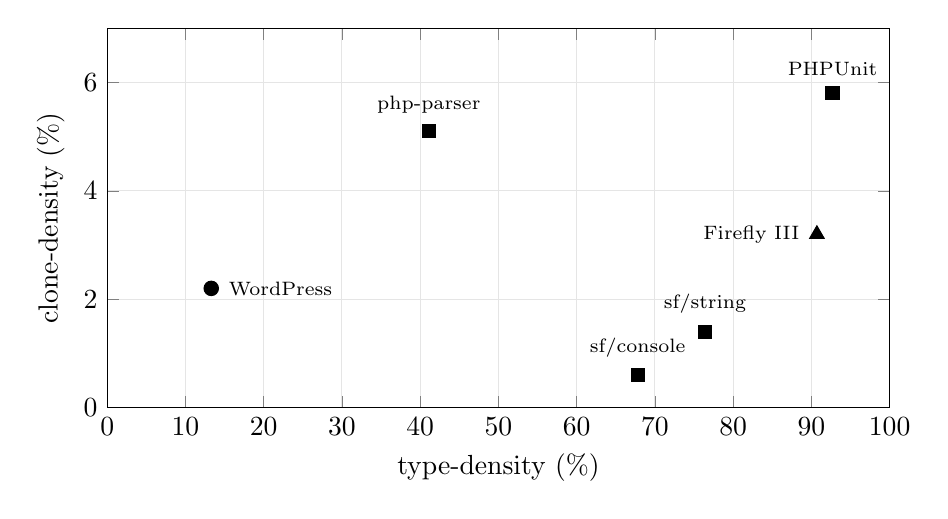
\begin{tikzpicture}
\begin{axis}[
  width=0.95\textwidth, height=6.4cm,
  xlabel={type-density (\%)}, ylabel={clone-density (\%)},
  xmin=0, xmax=100, ymin=0, ymax=7,
  grid=both, grid style={black!10},
  every node near coord/.append style={font=\scriptsize, anchor=south},
]
\addplot[only marks, mark=*,        mark size=2.6pt, black] coordinates {(13.3,2.2)};
\addplot[only marks, mark=square*,  mark size=2.4pt, black] coordinates {(41.1,5.1)(67.8,0.6)(76.4,1.4)(92.7,5.8)};
\addplot[only marks, mark=triangle*,mark size=3.0pt, black] coordinates {(90.7,3.2)};
\node[anchor=west,font=\scriptsize] at (axis cs:14.3,2.2) {WordPress};
\node[anchor=south,font=\scriptsize] at (axis cs:41.1,5.25) {php-parser};
\node[anchor=south,font=\scriptsize] at (axis cs:67.8,0.75) {sf/console};
\node[anchor=south,font=\scriptsize] at (axis cs:76.4,1.55) {sf/string};
\node[anchor=east,font=\scriptsize] at (axis cs:89.7,3.2) {Firefly III};
\node[anchor=south,font=\scriptsize] at (axis cs:92.7,5.95) {PHPUnit};
\legend{}
\end{axis}
\end{tikzpicture}
\caption{Type-density $\times$ clone-density map (full corpora, pinned SHAs).
Marks: $\bullet$~untyped control, $\blacksquare$~injection substrate,
$\blacktriangle$~ecological corpus. The scarce typed-and-cloney quadrant is occupied by an
application (Firefly~III), not a library.}
\label{fig:scatter}
\end{figure}

\begin{table}[h]
\centering
\caption{Computed type-density / clone-density map (\texttt{bench/measure-density.php}).}
\label{tab:density}
\small
\begin{tabular}{l r r r l}
\toprule
\textbf{corpus} & \textbf{files} & \textbf{type-dens.} & \textbf{clone-dens.} & \textbf{bucket} \\
\midrule
WordPress          & 1845 & 13.4\% & 2.2\% & untyped control \\
\texttt{nikic/php-parser} & 342 & 41.1\% & 5.1\% & injection (dependency) \\
\texttt{symfony/console} & \factScanSymfonyConsoleFiles & 67.8\% & 0.6\% & injection \\
\texttt{symfony/string} &  33 & 76.4\% & 1.4\% & injection \\
Firefly III        & \factScanFireflyIiiFiles & 90.7\% & 3.2\% & ecological \\
PHPUnit            & \factScanPhpunitFiles & 92.6\% & 5.7\% & injection (reflexive) \\
\bottomrule
\end{tabular}
\end{table}

\subsection{E2 --- the effect of type information}
The decisive operator, possible only in typed PHP, clones a block and changes an \texttt{int}-typed
variable to \texttt{string}-typed with structure held identical. Name-blind normalization calls these
clones (false positive); type-anchored normalization (\texttt{-{}-type-anchored}, which preserves
built-in type keywords instead of folding them to \texttt{ID}) correctly separates them. Injecting at
\emph{function} granularity over the full eligible population (functions carrying an
\texttt{int}/\texttt{float} hint, $\ge 25$ tokens), Figure~\ref{fig:lift} and Table~\ref{tab:e2}
report specificity.

\begin{figure}[h]
\centering
\begin{tikzpicture}
\begin{axis}[
  ybar,
  bar width=12pt,
  width=\textwidth, height=5.6cm,
  enlarge x limits=0.14,
  ymin=0, ymax=50,
  ylabel={specificity (\%)},
  symbolic x coords={symfony-string,symfony-console,phpunit,php-parser,wordpress},
  xtick=data,
  x tick label style={font=\footnotesize},
  nodes near coords, nodes near coords align={vertical},
  every node near coord/.append style={font=\scriptsize, text=black},
  legend style={at={(0.02,0.98)},anchor=north west,font=\footnotesize,draw=none},
]
\addplot+[ybar,pattern=north east lines,pattern color=black,draw=black] table[x=corpus,y=spec_anchored] {\etwodata};
\legend{\texttt{-{}-type-anchored} specificity}
\end{axis}
\end{tikzpicture}
\caption{Specificity on same-shape-different-type pairs. Name-blind \texttt{-{}-fuzzy} is a flat 0\%
floor (it calls every such pair a clone, so it is omitted from the bars); \texttt{-{}-type-anchored}
lifts specificity by $+1.9$ to $+18.9$ points at \emph{zero} recall cost (recall $=100\%$ in both
modes, Table~\ref{tab:e2}).}
\label{fig:lift}
\end{figure}

\begin{table}[h]
\centering
\caption{E2: type-anchored normalization over the full eligible-function population. Recall is identical in both modes;
the lift is pure specificity gain.}
\label{tab:e2}
\small
\pgfplotstabletypeset[
  col sep=tab,
  columns={corpus,pairs,spec_fuzzy,spec_anchored,lift,recall_anchored},
  columns/corpus/.style={string type,column name=\textbf{corpus},column type={l}},
  columns/pairs/.style={column name=\textbf{fns}},
  columns/spec_fuzzy/.style={fixed,zerofill,precision=1,column name=\makecell{\textbf{spec.}\\\textbf{fuzzy}}},
  columns/spec_anchored/.style={fixed,zerofill,precision=1,column name=\makecell{\textbf{spec.}\\\textbf{anchored}}},
  columns/lift/.style={fixed,zerofill,precision=1,column name=\textbf{lift}},
  columns/recall_anchored/.style={column name=\textbf{recall}},
  every head row/.style={before row=\toprule,after row=\midrule},
  every last row/.style={after row=\bottomrule},
]{\etwodata}
\end{table}

The lift is a property of \emph{type-load-bearing} functions, not of corpora: PHPUnit shows the
largest lift and php-parser one of the smallest, which inverts what an earlier measurement of this
experiment reported and is worth stating plainly. That measurement predates the change described in
\S\ref{sec:practical} that made single-character tokens visible to the matcher --- roughly half the
program text. A typed signature is a fixed number of tokens, so widening the stream it sits in makes
it a smaller share of every function, and type-anchoring has proportionally less to bite on: the lift
is real, dominance still holds, and it is smaller than it looked when operators were invisible.
php-parser feels that most because its node and visitor methods are short, so their signatures
carried the most weight before and lose the most now.
On the census the corpus-level
benefit no longer tracks type-density as it did (Pearson $r=0.43$, Spearman $\rho=0.30$ over the five
corpora): \texttt{symfony/string} is the second most densely typed and shows the smallest lift, while
WordPress is the least densely typed and shows more than php-parser. The scatter of
Figure~\ref{fig:scatter} is reported as the weak association it is rather than as a gradient, and the
per-corpus story still needs \emph{two} figures, because a lift concentrated in short typed functions
is not a property a single corpus-level number carries. Because the two modes share the same recall, this is a clean
dominance relation: on same-shape-different-type pairs, type-anchored normalization
\emph{Pareto-dominates} name-blind fuzzing --- equal recall at strictly higher specificity --- the
strongest form the claim can take, since here both axes are measured against injected ground truth.

\subsection{E3 --- inconsistent clones in practice}
\texttt{bench/run-e3.php} scans the ecological corpus (Firefly~III, 200 most-recently-modified files)
once through the suffix tree (\texttt{-{}-algorithm suffixtree -{}-edit-distance 3 -{}-min-tokens 50}), reads
the gapped clones via \lstinline!CodeClone::isGapped()! (the R4 capability), deduplicates by file
pair, and cross-references git: the \emph{staleness gap} is the number of days between the two copies'
last commits --- a high gap means one copy was maintained long after its sibling, the canonical
inconsistent-clone risk. The scan found 68 inconsistent clones and two distinct diverged-copy pairs
(Table~\ref{tab:e3}); both were manually verified as real. Exact-match output (Rabin--Karp /
\texttt{-{}-rk}) flags neither as inconsistent, having no gapped-clone concept.

\begin{table}[h]
\centering
\caption{E3 diverged-copy pairs in Firefly~III (200-file slice), ranked by staleness. Both verified
manually against source.}
\label{tab:e3}
\footnotesize
\begin{tabular}{@{}c p{2.6cm} p{2.6cm} c c p{4.0cm}@{}}
\toprule
\textbf{\#} & \textbf{copy A} & \textbf{copy B} & \textbf{lines} & \textbf{stale (d)} & \textbf{verdict} \\
\midrule
1 & \texttt{Navigation\-AddPeriodTest} & \texttt{Navigation\-PreferredSql\-FormatTest} & 4 & 35 &
Real --- duplicated \lstinline!setUp()! scaffold across two tests of the same class; a shared base
would remove it. \\
2 & \texttt{Autocomplete/\-CurrencyController} & \texttt{Autocomplete/\-TagController} & 25 & 9 &
Real --- identical DI constructor $+$ search loop; \texttt{Currency} later gained a deprecated
endpoint \texttt{Tag} never received. \\
\bottomrule
\end{tabular}
\end{table}

\section{Availability}
phpcpd-next is openly available under the permissive MIT licence. It began as a fork of
\texttt{sebastianbergmann/phpcpd}, archived in 2023 and then BSD~3-Clause; every
inherited file has since been rewritten from its specification, each proved to emit byte-identical
output before its attribution was changed, and \texttt{bench/check-provenance.php} measures that
inventory and reports it at zero. It has zero runtime dependencies (\texttt{php >=8.5} plus
\texttt{ext-dom}/\texttt{ext-mbstring}) and projects one format-neutral model
(\lstinline!CodeCloneMap!) to Text, PMD-CPD XML, JSON, and SARIF~2.1.0 --- the last ingested natively
by GitHub Code Scanning, with gapped (inconsistent) clones emitted at \texttt{warning} severity and
exact clones at \texttt{note}, so the bug-bearing clones surface as higher-severity PR annotations.
BCB-PHP ships as a fetch-script $+$ pinned SHAs $+$ injection manifests $+$ harness; every result is
reproducible from the SHAs and \texttt{composer.lock} files, and the modernization is recorded
diff-by-diff in \texttt{docs/MODERNIZATION.md}.

\section{Conclusion}
Starting from \texttt{phpcpd}'s Rabin--Karp exact matcher and its unreleased suffix-tree engine, we
asked an empirical question: of the clone-detection methods available, which are appropriate for a fast
PHP tool? Answering it required infrastructure that did not exist --- a labelled PHP clone benchmark ---
so we constructed one (BCB-PHP) while modernizing and completing the inherited engines and implementing
additional literature-grounded methods. The results --- a type-density gradient, a $+1.9$ to $+18.9$
point specificity increase from type-aware normalization at no recall cost, a six-corpus method
comparison, and confirmed inconsistent clones in an application corpus --- support a default that
combines exact and reorder-tolerant matching (\texttt{rk+tb}), retains fuzzing only for research, and
reserves approximate suffix-tree matching for targeted analysis. Those three engines became
the \emph{measured baselines} for a fourth (\S\ref{sec:unified}) that subsumes what each was kept for:
exact matching, reorder tolerance, and gapped matching with the divergent ranges named rather than a
boolean. Which of them a release ships as the default was put to a criterion fixed before the
measurement, and answered: the criterion is not met
(\S\ref{sec:precision-correction}), the merged pipeline remains the default, and the suffix-tree
engine --- the one component of the package that was not its authors' own work --- was removed in
\factCodeRelease{} once the fourth engine covered what it was kept for.

\paragraph{Future work.} The component most likely to outlast any single result is the benchmark, since
it turns open questions about PHP clone detection from matters of argument into measurable ones. Three
directions follow from the evidence. First, the injection operators can be broadened beyond the
\texttt{int}/\texttt{float} confusion studied here to a wider class of type-level edits
(\texttt{bool}$\leftrightarrow$\texttt{int}, nullable versus non-nullable, and class or interface
substitutions), enlarging the type-load-bearing population and testing whether the specificity gain of
type-anchored normalization generalizes across type kinds. Second, the harness can be applied to
further real-world and proprietary codebases to assess external validity beyond the six public corpora.
Third, the residual cost of suffix-tree matching --- candidate enumeration, the part the banded DP
(\S\ref{sec:practical}) does not reduce --- was the engine's main scaling limit on large corpora, and
\S\ref{sec:unified} reports what replaced it: enumeration became a sample with a proof attached
rather than an exhaustive pass to be optimized. What remains open there is not enumeration but
verification cost on self-similar files, and the precision boundary of
\S\ref{sec:precision-correction} --- a residue that three rating rounds have located in the raters'
own disagreement rather than in any mechanical rule, which suggests the next instrument should
measure a \emph{ranked} report rather than a flat pool. In each case the methodological commitment is
the one adopted throughout: a candidate improvement is admitted on PHP-specific empirical evidence, not on
its theoretical appeal.

\begin{thebibliography}{99}
\small
\bibitem{roycordy} C.~K. Roy and J.~R. Cordy, ``A survey on software clone detection research,''
Queen's Univ.\ Tech.\ Rep.\ 2007-541, 2007.

\bibitem{conqat} E.~Juergens, F.~Deissenboeck, B.~Hummel, and S.~Wagner, ``Do code clones matter?''
in \emph{Proc.\ ICSE}, 2009, pp.~485--495.

\bibitem{sourcerercc} H.~Sajnani, V.~Saini, J.~Svajlenko, C.~K. Roy, and C.~V. Lopes,
``SourcererCC: scaling code clone detection to big-code,'' in \emph{Proc.\ ICSE}, 2016,
pp.~1157--1168. arXiv:1512.06448, 1603.01661.

\bibitem{toma} Y.~Wu \emph{et al.}, ``Toma: a token-type-aware clone detector'' (token-type
abstraction, six similarity measures, ``simple clones dominate''), in \emph{Proc.\ ICSE}, 2024.

\bibitem{hummel} B.~Hummel, E.~Juergens, L.~Heinemann, and M.~Conradt, ``Index-based code clone
detection: incremental, distributed, scalable,'' in \emph{Proc.\ ICSM}, 2010, pp.~1--9.

\bibitem{deckard} L.~Jiang, G.~Misherghi, Z.~Su, and S.~Glondu, ``DECKARD: scalable and accurate
tree-based detection of code clones,'' in \emph{Proc.\ ICSE}, 2007, pp.~96--105.

\bibitem{winnowing} S.~Schleimer, D.~S. Wilkerson, and A.~Aiken, ``Winnowing: local algorithms for
document fingerprinting,'' in \emph{Proc.\ SIGMOD}, 2003, pp.~76--85.

\bibitem{sparse} D.~Eppstein, Z.~Galil, R.~Giancarlo, and G.~F. Italiano, ``Sparse dynamic
programming I: linear cost functions,'' \emph{J.\ ACM}, vol.~39, no.~3, pp.~519--545, 1992.

\bibitem{broder} A.~Z. Broder, ``On the resemblance and containment of documents,'' in
\emph{Proc.\ Compression and Complexity of Sequences}, 1997, pp.~21--29.

\bibitem{prefixfilter} S.~Chaudhuri, V.~Ganti, and R.~Kaushik, ``A primitive operator for
similarity joins in data cleaning,'' in \emph{Proc.\ ICDE}, 2006, p.~5.

\bibitem{ppjoin} C.~Xiao, W.~Wang, X.~Lin, J.~X. Yu, and G.~Wang, ``Efficient similarity joins for
near-duplicate detection,'' \emph{ACM Trans.\ Database Syst.}, vol.~36, no.~3, pp.~1--41, 2011.

\bibitem{bigclonebench} J.~Svajlenko, J.~F. Islam, I.~Keivanloo, C.~K. Roy, and M.~M. Mia,
``Towards a big data curated benchmark of inter-project code clones,'' in \emph{Proc.\ ICSME}, 2014,
pp.~476--480.
\end{thebibliography}

\end{document}
